\section[Intuition et définitions]{Intuition et définitions}

\subsection[Intuition]{Intuition}

\begin{frame}{Présentation du cas d'étude}
	Nous considérerons le cas d'étude suivant:
	\begin{itemize}
		\item Supposons que nous voulions connaitre la taille moyenne des individus sur le campus de l'Université de Toulouse 3.
		\pause
		\item Il existe une valeur \textbf{vraie}. C'est la valeur que l'on obtiendrait si on mesurait \textit{tout le monde}.
		\pause
		\item En pratique, on travaillera avec des \textbf{échantillons}.
	\end{itemize}
\end{frame}

\begin{frame}{Construction des intervalles}
	Pour l'intervalle de prédiction:
	\begin{itemize}
		\item On collecte les tailles de $n$ étudiant(e)s.
		\item On cherche un estimateur de maximum de vraisemblance pour les \textbf{tailles} avec une distribution Gaussienne.
		\item On calcule l'intervalle centré représentant 95\% des \textbf{tailles} mesurées.
	\end{itemize}
	\pause
	Pour l'intervalle de confiance:
	\begin{itemize}
		\item On génère $m$ échantillons:
		\begin{itemize}
			\item On collecte les tailles de $n$ étudiant(e)s.
			\item On calcule la taille moyenne de l'échantillon.
		\end{itemize}		
		\item On cherche un estimateur de maximum de vraisemblance pour les \textbf{moyennes} avec une distribution Gaussienne.
		\item On calcule l'intervalle centré représentant 95\% des \textbf{moyennes} mesurées.
	\end{itemize}
\end{frame}

\begin{frame}{Résultats avec $n = 30$ et $m = 100$}
	\begin{columns}
		\begin{column}{0.5\textwidth}
			\begin{figure}
				\centering
				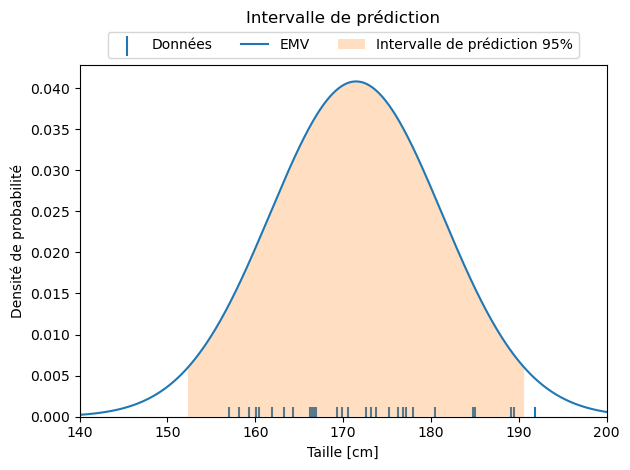
\includegraphics[width=1.0\linewidth]{Images/intervalle_prediction_n30}
				\label{fig:intervalle-prediction-n30}
			\end{figure}
		\end{column}
		\begin{column}{0.5\textwidth}
			\begin{figure}
				\centering
				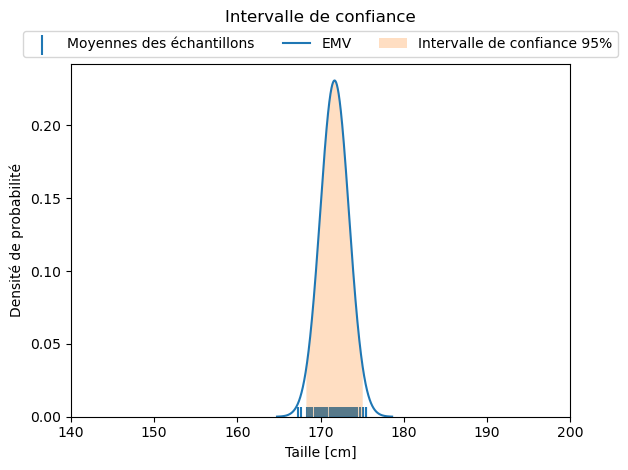
\includegraphics[width=1.0\linewidth]{Images/intervalle_confiance_n30}
				\label{fig:intervalle-confiance-n30}
			\end{figure}
		\end{column}
	\end{columns}
\end{frame}

\begin{frame}{Résultats avec $n = 300$ et $m = 100$}
	\begin{columns}
		\begin{column}{0.5\textwidth}
			\begin{figure}
				\centering
				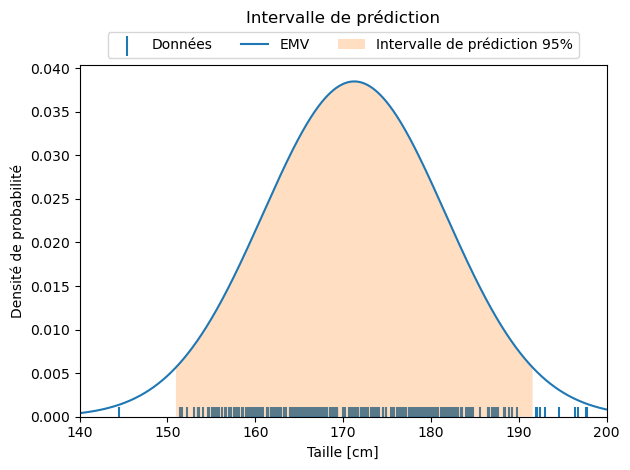
\includegraphics[width=1.0\linewidth]{Images/intervalle_prediction_n300}
				\label{fig:intervalle-prediction-n300}
			\end{figure}
		\end{column}
		\begin{column}{0.5\textwidth}
			\begin{figure}
				\centering
				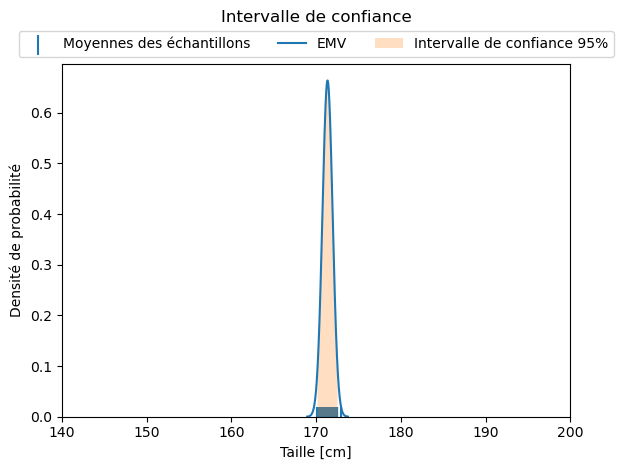
\includegraphics[width=1.0\linewidth]{Images/intervalle_confiance_n300}
				\label{fig:intervalle-confiance-n300}
			\end{figure}
		\end{column}
	\end{columns}
\end{frame}

\begin{frame}{Discussion}
	\begin{itemize}
		\item L'intervalle de prédiction ne change que très légèrement en augmentant la taille de l'échantillon.
		\item L'intervalle de confiance se resserre en augmentant la taille d'échantillon.
		\item L'intervalle de prédiction mesure la disparité de taille au sein d'un échantillon.
		\item L'intervalle de confiance mesure la disparité de la moyenne de plusieurs échantillons.
	\end{itemize}
	\pause
	\vspace{0.5cm}
	L'écart type de l'intervalle de confiance, appelé \textbf{erreur type} ($\ET$), se réduit quand la taille de l'échantillon augmente. Il varie en $1 / \sqrt{n}$.
\end{frame}

\begin{frame}{Interprétation}
	\begin{itemize}
		\item Un intervalle de prédiction à 95\% signifie que 95\% des futures observations se situeront dans cet intervalle.
		\pause
		\item Un intervalle de confiance à 95\% signifie que 95\% des futures moyennes d'échantillons, calculées d'une manière identique, se situeront dans cet intervalle.
		\pause
		\item Attention, la couverture de 95\% n'est pas \textbf{garantie}. Elle dépend de la validité des hypothèses, notamment de la nature Gaussienne des distributions.
	\end{itemize}
	\pause
	Si l'écart type de la taille d'un groupe d'étudiants $\sigma$ est connue, l'erreur type $\ET$ peut se calculer à partir de la taille d'échantillon $n$:
	\begin{equation}
		\ET = \frac{\sigma}{\sqrt{n}}
		\nonumber
	\end{equation}
\end{frame}